\subsubsection{1.2. Mô hình MGAT + FastKAN/MLP}

\begin{figure}[H]
    \centering
    \scalebox{0.4}{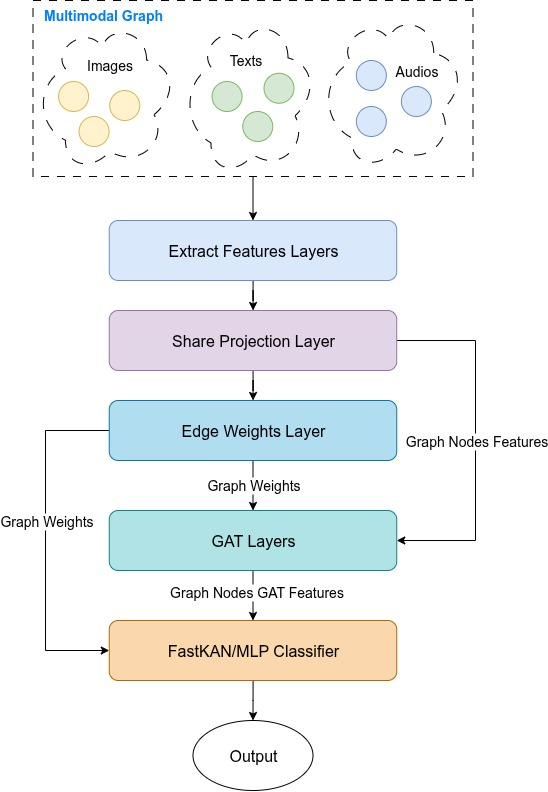
\includegraphics[width=\linewidth]{images/part-02/chap-02/sec-01/Pipeline.jpg}}
    \vspace{0.3cm}
    \caption{Kiến trúc tổng quát của mô hình CNN backbone + MGAT + FastKAN/MLP}
    \label{fig:KTPipeline}
\end{figure}

\begin{figure}[H]
    \centering
    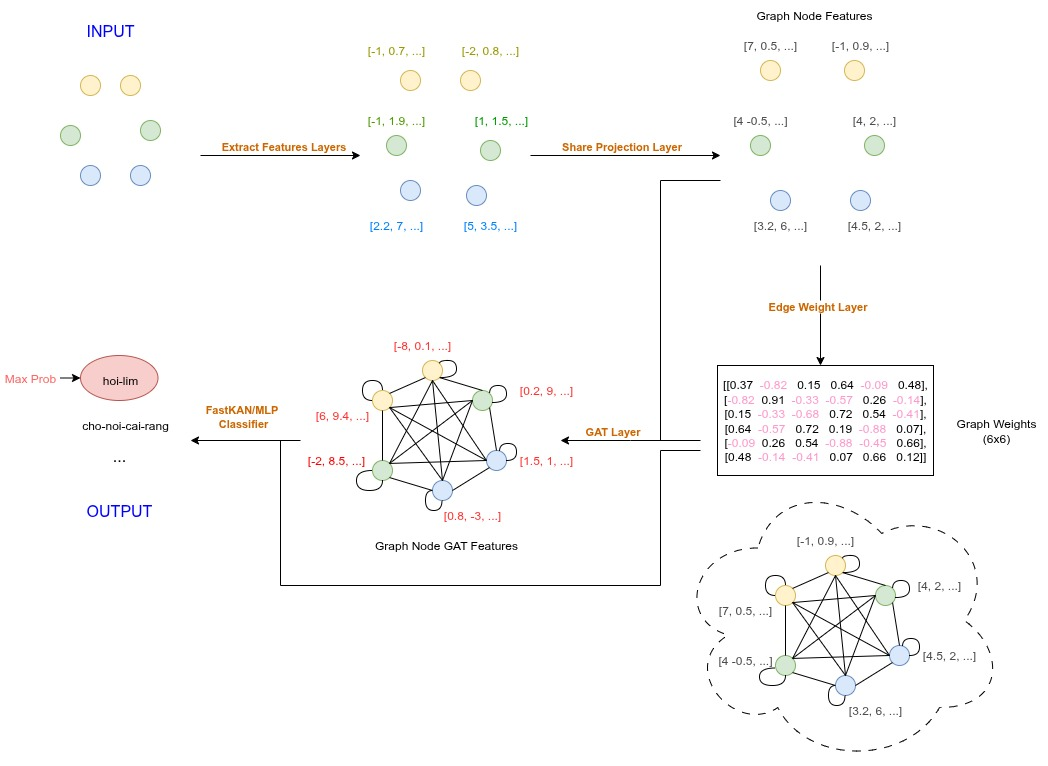
\includegraphics[width=\linewidth]{images/part-02/chap-02/sec-01/ViDuDoThi.jpg}
    \vspace{0.3cm}
    \caption{\centering Ví dụ về cách xây dựng đồ thị và dự đoán nhãn khi dùng mô hình CNN backbone + MGAT + FastKAN/MLP}
    \label{fig:VDPipeline}
\end{figure}

% \indent\indent Kiến trúc của mô hình gồm 5 tầng được mô tả tổng quát qua \textbf{Hình} \ref{fig:KTPipeline} và có ví dụ cụ thể ở \textbf{Hình} \ref{fig:VDPipeline}, trong đó mỗi tầng làm nhiệm vụ cụ thể như sau:
% \begin{itemize}
%     \item \textbf{Extract Features Layers:} Tầng dùng để trích xuất đặc trưng riêng biệt cho từng loại phương thức, như ví dụ ở \textbf{Hình} \ref{fig:VDPipeline}, khi đồ thị ban đầu đi qua tầng này, ta được các đặc trưng ở không gian khác nhau tuỳ thuộc phương thức của nút đó (nút màu vàng là hình ảnh, nút màu xanh lá là văn bản, nút màu xanh dương là âm thanh).
%     \item \textbf{Share Projection Layer:} Tầng biến đổi không gian từ các phương thức khác nhau về cùng một không gian chung để chúng được biểu diễn một cách thống nhất.
%     \item \textbf{Edge Weight Layer}: Tầng này dùng các vector ở các nút do Share Projection Layer sinh ra để tiến hành tính trọng số trên cạnh, là một bộ trọng số vô hướng có giá trị từ $[-1, 1]$, nhằm mục tiêu là học mối quan hệ "bạn bè" (trọng số cạnh dương) hoặc "đối kháng" (trọng số cạnh âm) giữa các nút.
%     \item \textbf{GAT Layer}: Tầng ứng dụng GAT để tổng hợp vector mới cho các nút từ thông tin các nút hàng xóm của nó, ở đây ta chỉ xét các hàng xóm thuộc nhóm "bạn bè", vì chúng là những hàng xóm mang thông tin bổ sung cần thiết cho nút hiện tại.
%     \item \textbf{FastKAN/MLP Classifier}: Tầng này sử dụng vector mới từ GAT Layer để tiến hành phân lớp, bằng cách đem các nút đi dự đoán, và cộng trung bình dự đoán có trọng số của các nút (bằng cách Graph Weight từ tầng Edge Weight Layer) nhằm tăng tính linh hoạt của mô hình, mỗi nút sẽ có đóng góp khác nhau vào kết quả cuối cùng.
% \end{itemize}

\indent\indent Kiến trúc của mô hình gồm 5 tầng, được mô tả tổng quát trong \textbf{Hình} \ref{fig:KTPipeline} và được minh hoạ cụ thể qua \textbf{Hình} \ref{fig:VDPipeline}. Mỗi tầng đảm nhận một vai trò riêng trong toàn bộ pipeline, cụ thể như sau:
\begin{itemize}[label={--}, itemsep=1pt]
    \item \textbf{Extract Features Layers:} Tầng này có nhiệm vụ trích xuất đặc trưng riêng cho từng loại phương thức dữ liệu. Như minh hoạ trong \textbf{Hình} \ref{fig:VDPipeline}, khi đồ thị ban đầu đi qua tầng này, các nút sẽ được ánh xạ sang những không gian đặc trưng khác nhau tuỳ theo phương thức của chúng (nút màu vàng biểu diễn hình ảnh, nút màu xanh lá biểu diễn văn bản, và nút màu xanh dương biểu diễn âm thanh).
    
    \item \textbf{Share Projection Layer:} Tầng này thực hiện phép chiếu các đặc trưng từ những không gian phương thức khác nhau về một không gian biểu diễn chung, nhằm đảm bảo các nút được biểu diễn một cách thống nhất và có thể so sánh trực tiếp với nhau.
    
    \item \textbf{Edge Weight Layer}: Dựa trên các vector biểu diễn của nút do Share Projection Layer sinh ra, tầng này học và tính toán trọng số cho các cạnh trong đồ thị. Trọng số cạnh là một giá trị nằm trong đoạn $[-1, 1]$, phản ánh mức độ quan hệ giữa các nút, trong đó trọng số dương biểu thị mối quan hệ "bạn bè", còn trọng số âm biểu thị mối quan hệ "đối kháng".
    
    \item \textbf{GAT Layers}: Tầng này áp dụng GAT để tổng hợp và cập nhật biểu diễn mới cho mỗi nút dựa trên thông tin từ các nút hàng xóm. Trong quá trình này, mô hình chỉ xét các hàng xóm có trọng số cạnh dương (nhóm "bạn bè"), vì đây là những nút cung cấp thông tin bổ trợ hữu ích cho nút đang xét.
    
    \item \textbf{FastKAN/MLP Classifier}: Tầng này sử dụng các vector đã được cập nhật từ GAT Layer để thực hiện phân lớp. Đầu tiên, mô hình tiến hành dự đoán trên từng nút và sau đó tổng hợp kết quả bằng cách lấy trung bình có trọng số, trong đó trọng số được xác định bởi Graph Weight từ Edge Weight Layer. Phương pháp này giúp tăng tính linh hoạt của mô hình, cho phép mỗi nút đóng góp khác nhau vào kết quả dự đoán cuối cùng.
\end{itemize}


\paragraph{1.2.1. Extract Features Layers (Tầng trích xuất đặc trưng)}
\indent\indent Đây là tầng nhận dữ liệu đồ thị từ ba phương thức khác nhau. Kiến trúc của tầng này được minh họa tại \textbf{Hình \ref{fig:KTExtractFeaturesLayers}}, bao gồm ba nhánh xử lý độc lập:\vspace{-0.1cm}
\begin{itemize}[label={--}, itemsep=1pt]
    \item Extract Image Features Layer: Sử dụng backbone CNN đã được đóng băng tham số và BatchNorm để trích xuất đặc trưng hình ảnh. Đầu ra từ backbone được đưa qua một tầng Linear để chiếu về chiều không gian vector mong muốn (448 chiều).
    \item Extract Text Features Layer: Kết hợp vector embedding của từ (Word) và câu (Sentence).
    \item Extract Audio Features Layer: Xử lý đặc trưng MFCC kết hợp với các giá trị Delta và Delta-Delta.
\end{itemize}

\begin{figure}[H]
    \centering
    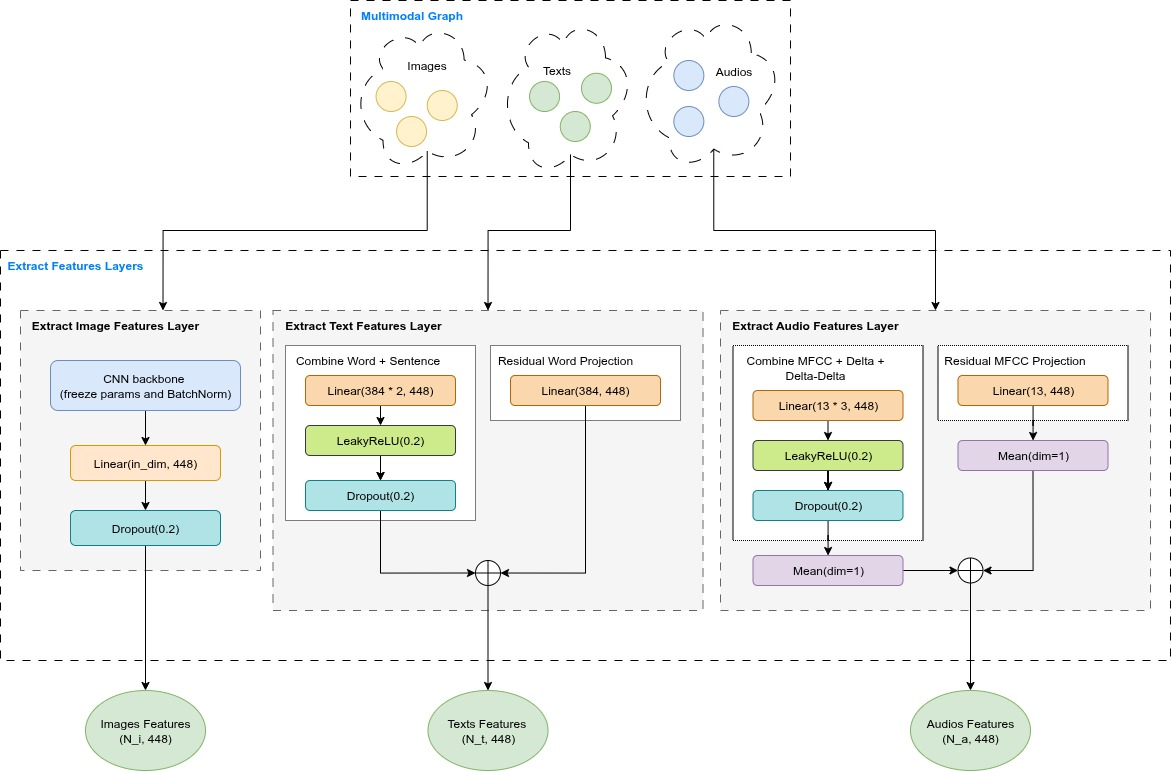
\includegraphics[width=\linewidth]{images/part-02/chap-02/sec-01/ExtractFeaturesLayers.jpg}
    \vspace{0.3cm}
    \caption{Kiến trúc chi tiết của Extract Features Layers}
    \label{fig:KTExtractFeaturesLayers}
\end{figure}

Đối với nhánh đặc trưng hình ảnh, do backbone đã cung cấp các vector đặc trưng giàu thông tin ngữ nghĩa, mô hình chỉ áp dụng phép chiếu tuyến tính đơn giản. Ngược lại, đối với văn bản và âm thanh, mô hình áp dụng cơ chế Residual Connection bằng cách cộng vector đặc trưng gốc (đã được chiếu về cùng chiều) vào đầu ra cuối cùng của nhánh. Kỹ thuật này giúp giải quyết vấn đề biến mất đạo hàm khi huấn luyện mạng sâu, đồng thời bảo toàn thông tin gốc quan trọng trước các phép biến đổi phi tuyến có thể gây mất mát thông tin đặc trưng \cite{he2015deepresiduallearningimage}.
\paragraph{1.2.2. Share Projection Layer (Tầng chiếu không gian chung)}
\indent\indent Mục tiêu của tầng này là đồng bộ hóa các vector đặc trưng từ ba phương thức khác nhau về cùng một không gian biểu diễn có số chiều cố định (512 chiều), với kiến trúc chi tiết tại \textbf{Hình \ref{fig:KTShareProjectionLayer}}.

\begin{figure}[H]
    \centering
    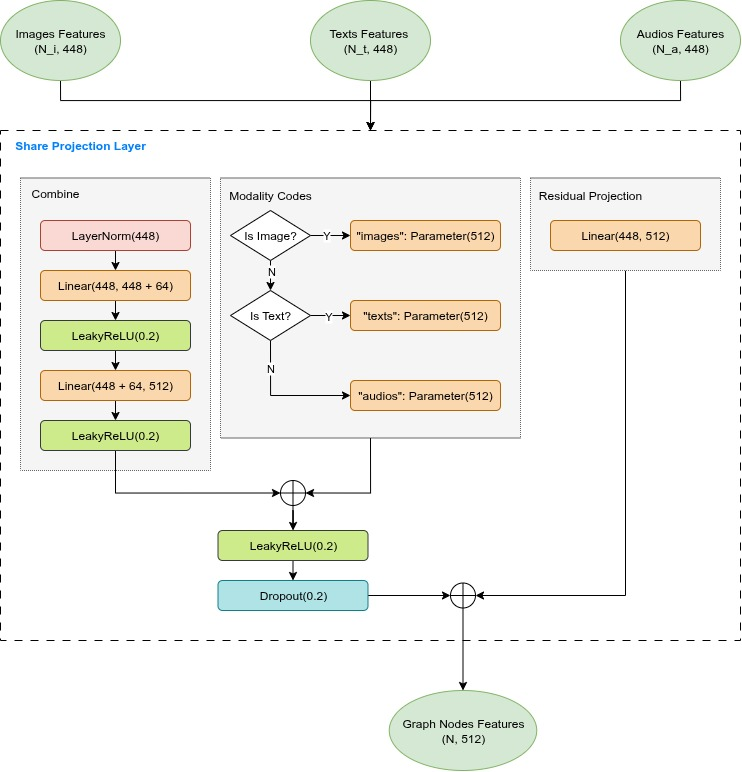
\includegraphics[width=0.8\linewidth]{images/part-02/chap-02/sec-01/ShareProjectionLayer.jpg}
    \vspace{0.3cm}
    \caption{Kiến trúc của Share Projection Layer}
    \label{fig:KTShareProjectionLayer}
\end{figure}

Để phân biệt được phương thức của từng vector đặc trưng trong không gian chung, mô hình sử dụng kỹ thuật Modality Embeddings (hay Modality Codes). Mỗi phương thức được gán một vector tham số học được riêng biệt, cộng trực tiếp vào đặc trưng đầu ra nhằm "đánh dấu" vị trí của nó trong không gian vector chung. Kỹ thuật này được lấy cảm hứng từ cơ chế Token Type Embeddings trong mô hình BERT, giúp mô hình nhận biết ngữ cảnh phương thức \cite{devlin2019bertpretrainingdeepbidirectional}. Đồng thời, cơ chế Residual Connection tiếp tục được áp dụng tại đây nhằm duy trì luồng thông tin xuyên suốt, tránh sự mất mát dữ liệu do các phép biến đổi của tầng Linear.
\paragraph{1.2.3. Edge Weight Layer (Tầng học trọng số cạnh)}
\indent\indent Tầng này đóng vai trò khởi tạo cấu trúc đồ thị bằng cách xác định độ mạnh yếu của các liên kết giữa các đỉnh, như minh họa tại \textbf{Hình \ref{fig:KTEdgeWeightsLayer}}.

\begin{figure}[H]
    \centering
    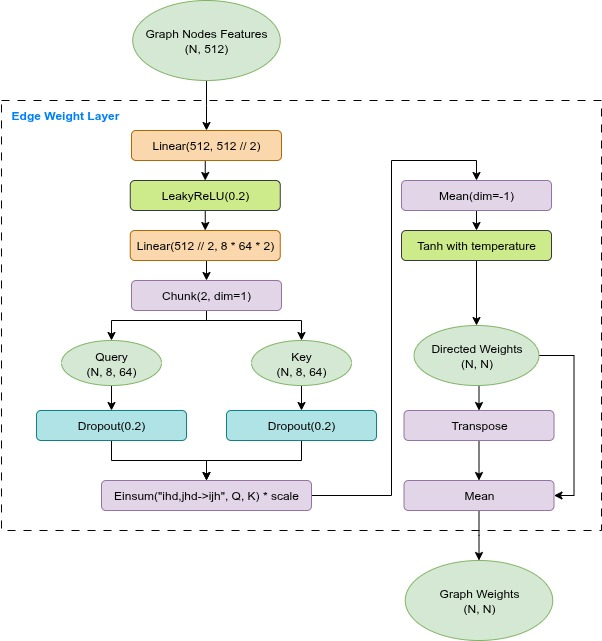
\includegraphics[width=0.8\linewidth]{images/part-02/chap-02/sec-01/EdgeWeightsLayer.jpg}
    \vspace{0.3cm}
    \caption{Kiến trúc của Edge Weights Layer sử dụng cơ chế Attention}
    \label{fig:KTEdgeWeightsLayer}
\end{figure}

\indent Mạng học trọng số cạnh được xây dựng dựa trên cơ chế \textit{self-attention}, trong đó tích vô hướng $Q \cdot K^{T}$ được sử dụng để thể hiện tính tương quan ngữ nghĩa giữa các nút \cite{vaswani2023attentionneed}. Đầu ra của tầng này sử dụng hàm kích hoạt \texttt{Tanh} nhằm giới hạn giá trị trọng số cạnh trong khoảng $[-1, 1]$, điều này cho phép mô hình biểu diễn hai loại quan hệ đối lập: quan hệ "bạn bè" với trọng số cạnh dương (tiệm cận 1) và quan hệ "đối kháng" với trọng số cạnh âm (tiệm cận $-1$).\vspace{0.3cm}

Việc cho phép tồn tại trọng số cạnh âm ở giai đoạn này đóng vai trò như một cơ chế lọc mềm. Với các giá trị trọng số âm sẽ được loại bỏ ở các tầng tiếp theo thông qua hàm \texttt{Clamp(min=0)}, nhờ đó mô hình có khả năng chủ động học cách loại bỏ các kết nối nhiễu hoặc không mang thông tin hữu ích. Phương pháp này linh hoạt hơn so với việc sử dụng hàm kích hoạt \texttt{Sigmoid}, vốn chỉ sinh ra các trọng số không âm trong khoảng $(0,1)$, điều này buộc mô hình phải duy trì tất cả các cạnh với mức độ ảnh hưởng khác nhau, kể cả những kết nối kém liên quan (có trọng số dương rất nhỏ, tiệm cận 0).\vspace{0.3cm}

Ngoài ra, để đảm bảo tính vô hướng của đồ thị, chỉ cần lấy ma trận trọng số cạnh tính được đem trung bình cộng với ma trận chuyển vị của chính nó. Cách xử lý này đảm bảo rằng trọng số liên kết giữa hai nút là nhất quán theo cả hai chiều, tức trọng số từ nút $A$ đến nút $B$ bằng với trọng số từ $B$ đến $A$.

\paragraph{1.2.4. GAT Layers (Tầng GAT)}
\indent\indent Đây là thành phần cốt lõi thực hiện quá trình truyền tin (Message Passing) để cập nhật đặc trưng nút, với kiến trúc được minh hoạ như \textbf{Hình \ref{fig:KTGATLayers}}.

\begin{figure}[H]
    \centering
    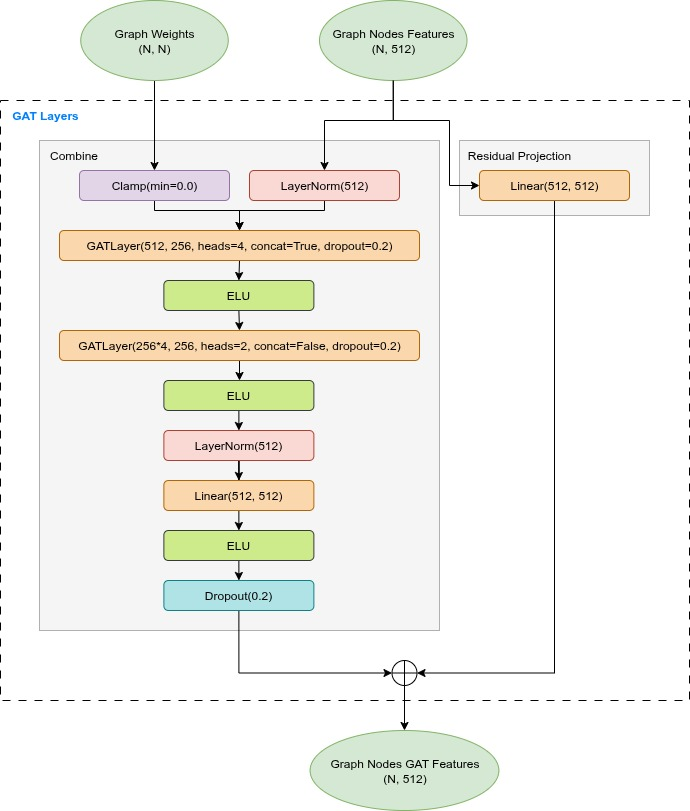
\includegraphics[width=0.8\linewidth]{images/part-02/chap-02/sec-01/GATLayers.jpg}
    \vspace{0.3cm}
    \caption{Kiến trúc của GAT Layers với cơ chế Weighted Message Passing}
    \label{fig:KTGATLayers}
\end{figure}

Mô hình áp dụng biến thể Weighted GAT kết hợp với Dynamic Attention. Khác với GAT truyền thống chỉ dựa vào đặc trưng nút và ma trận kề để tính hệ số attention, thì mô hình trong đề tài này tích hợp trực tiếp trọng số cạnh học được ($GW_{ij}$) vào quá trình tính toán, với công thức cụ thể như sau:
\[
    \alpha_{ij} = \text{softmax}(\text{LeakyReLU}(\vec{a}^T [W\vec{h}_i \| W\vec{h}_j]) \cdot {GW}_{ij})
\]
\indent Trong đó $GW_{ij}$ là ma trận trọng số cạnh của đồ thị từ tầng trước đã qua hàm \texttt{Clamp(min=0.0)} để loại bỏ giá trị âm. Cơ chế này giúp khắc phục hạn chế "Static Attention", cho phép mô hình kiểm soát luồng thông tin linh hoạt hơn: các cạnh có trọng số lớn sẽ khuếch đại tín hiệu, ngược lại các cạnh yếu sẽ bị chặn lại. Hàm kích hoạt phi tuyến ELU (Exponential Linear Unit) được sử dụng sau mỗi lớp GAT nhằm hỗ trợ việc học các biểu diễn của vector tốt hơn và tăng tốc độ hội tụ so với ReLU thông thường \cite{clevert2016fastaccuratedeepnetwork}.\vspace{0.3cm}

Ngoài ra, tầng này cũng được áp dụng thêm kỹ thuật Pre-LayerNorm (chuẩn hóa trước khi đưa vào layer) để ổn định gradient khi huấn luyện mô hình sâu, tránh hiện tượng bùng nổ hoặc biến mất gradient thường gặp trong các mạng GNN nhiều lớp \cite{xiong2020layernormalizationtransformerarchitecture}. Tương tự các tầng trước, cơ chế Residual Connection vẫn được duy trì để bảo toàn thông tin gốc qua các phép biến đổi phức tạp.
\paragraph{1.2.5. FastKAN/MLP Classifier (Bộ phân lớp)}
\indent\indent Tầng cuối cùng thực hiện ánh xạ từ không gian đặc trưng đồ thị sang không gian nhãn xác suất, sử dụng FastKAN hoặc MLP như minh họa tại \textbf{Hình \ref{fig:KTClassifier}}.

\begin{figure}[H]
    \centering
    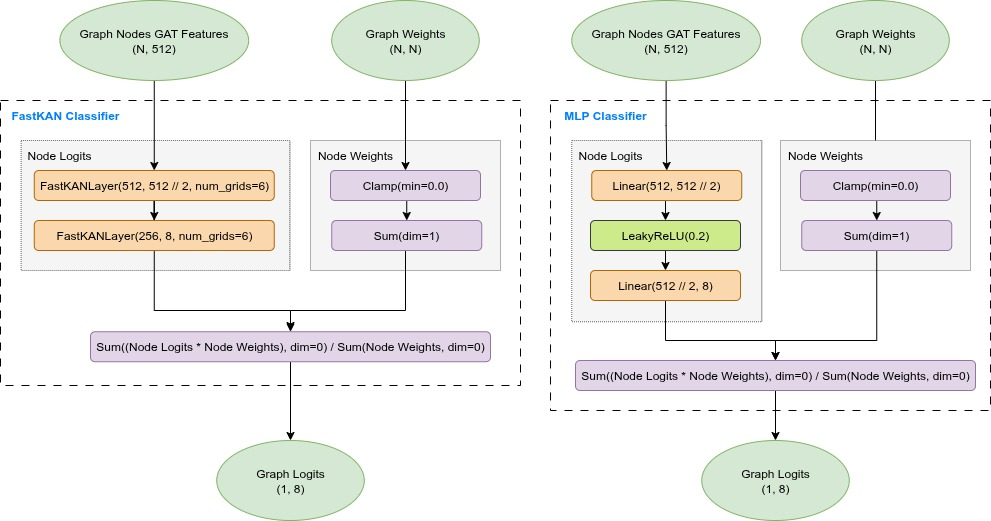
\includegraphics[width=\linewidth]{images/part-02/chap-02/sec-01/Classifier.jpg}
    \vspace{0.3cm}
    \caption{Kiến trúc bộ phân lớp bằng FastKAN và MLP}
    \label{fig:KTClassifier}
\end{figure}

Thay vì sử dụng kỹ thuật Global Mean Pooling thông thường (coi vai trò các nút là như nhau), mô hình áp dụng cơ chế Weighted Pooling (trung bình có trọng số). Kết quả dự đoán cuối cùng là trung bình có trọng số của các dự đoán từ từng nút ($logits_i$), với trọng số của mỗi nút được tính dựa trên tổng trọng số cạnh dương ($d_i = \sum_j w_{ij}$) của nút đó, với công thức cụ thể như sau:
\[
    y_{pred} = \frac{\sum_i (logits_i \cdot d_i)}{\sum_i d_i + \epsilon}
\]
\indent Trong đó $\epsilon$ là hằng số nhỏ để tránh lỗi chia cho 0. Cơ chế này phù hợp với lý thuyết về Graph Readout Operations, khẳng định rằng việc tổng hợp thông tin dựa trên cấu trúc giúp mô hình ưu tiên các nút giàu thông tin và giảm thiểu tác động của các nút ngoại lai lên kết quả dự đoán cuối cùng \cite{xu2019powerfulgraphneuralnetworks}.
